\documentclass[10pt, twocolumn, twoside]{article}
\usepackage[T1]{fontenc}
\usepackage{cuted}
\usepackage{graphicx}
\usepackage{bm}
\usepackage{geometry}
\usepackage{bbm}
\geometry{a4paper,total={170mm,257mm},left=20mm,top=20mm,}
\pagenumbering{arabic}
\usepackage{hyperref}
\usepackage{url}
\usepackage{scrextend}
\usepackage{amsmath,amssymb}
\usepackage{ragged2e}
\setcounter{tocdepth}{1}
%\usepackage[backend=biber,style=nature,sorting=nyt]{biblatex}
%\addbibresource{su4.bib}

\title{Quantum Monte Carlo Simulations of the Hubbard model}
\author{Francisco Monteiro de Oliveira Brito}
\date{\today}
\setlength\columnsep{1.5em}

\makeatletter

\begin{document}

\begin{strip}
\vspace*{\dimexpr-\baselineskip-\stripsep\relax}
\centering
\maketitle
\vskip\baselineskip
\noindent%\makebox[\textwidth]{\rule{1.1\paperwidth}{0.4pt}}
\vskip\baselineskip
\justify
\begin{abstract}\paragraph{}
TO DO
\end{abstract}
\end{strip}

\section{Introduction}\paragraph{}

We start with an overview of the Hubbard model and in section \ref{hubbQMC} we provide details on how to simulate it numerically using quantum Monte Carlo. The reader who is already familiar with the Hubbard model can safely skip this introductory section. The Hubbard model appeared as one of the first attempts to include electron correlation effects in a quantum mechanical description of a solid. Originally, it was introduced to explain the behavior of the electrons occupying the narrow, partly filled $d-$bands of transition metals. Correlation phenomena in these bands lead to a behavior reminiscent of the atomic picture of a solid. 

The free (or \emph{nearly} free) electron gas models the conduction bands of metals and alloys fairly accurately. However, in transition and rare-earth metals, in addition to the conduction bands, there are partially filled $d-$ or $f-$bands which are responsible for the characteristic properties of these solids. In these narrow energy bands correlation phenomena are particularly relevant, as opposed to the case of conduction bands. Thus, the free electron gas model does not suffice to describe the electrons in these bands; we must turn to a model that includes correlations. While for $f-$electrons of rare earth metals, a purely atomic, localized model - such as the Heitler-London model - might be satisfactory, the same cannot be said for $d-$electrons of transition metals.

First, note that the effects of correlations cannot possibly be the same in narrow energy bands and in the (nearly) free electron gas. To see this, we may simply  recall the shape of a $d-$wave function. In a $d-$orbital, the electron charge density is concentrated near the nuclei of the solid\footnote{The electronic charge density is, of course, not actually defined in terms of a squared norm of the $d-$wave function for a narrow band. There is some broadening of the corresponding atomic energy level, and the wave function describing an electron is a Bloch wave function. Since the band is narrow, we assume that the atomic wave function description is still somewhat useful in a given range and we use it to provide a heuristic motivation for the non validity of the free electron assumption.}. It is much smaller between atoms so that electrons do seem to belong to individual atoms in some sense. For a $d-$band, we assume that the case is not so different since the band is narrow. The fact that we may speak with some meaning of an electron belonging to a particular atom motivates an atomic description, in spite of the fact that the bandwidth of a $d-$band is still appreciable. The point is that electrons in $d-$bands are certainly not well described by a free electron gas.

\begin{figure}[ht!]
\centering
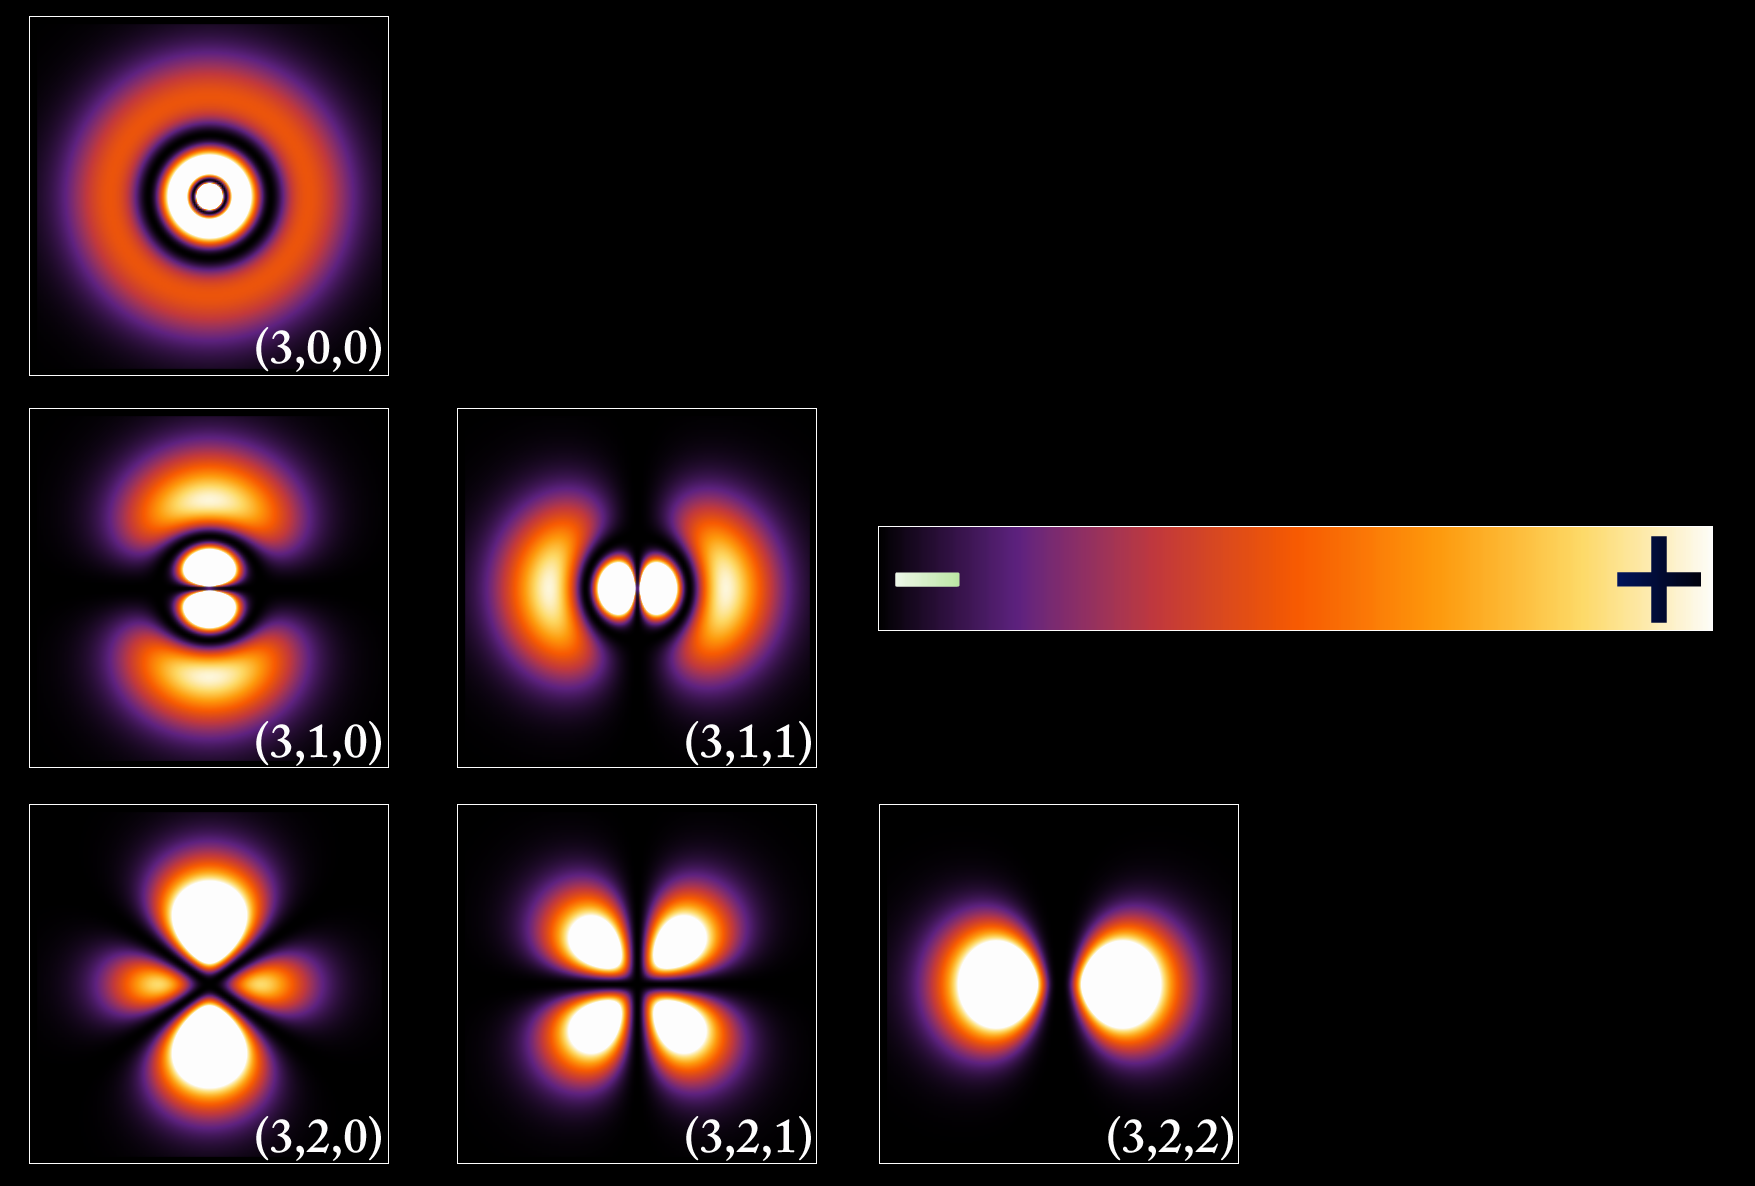
\includegraphics[width = 8.2cm]{Hydrogen_Density_Plots.png}
\caption{Probability density plots for different hydrogen orbital wave functions corresponding to quantum numbers $(n, l, m)$. d-wave functions correspond to $l=2$. Note that the probability density is always higher in a region near the nucleus, and has a complicated shape, which will lead to a highly non-uniform distribution of electronic charge.}
\end{figure}

Experimentally, $d-$electrons of transition metals show a hybrid behavior: sometimes they are accurately described by an ordinary band model, but there are occasions in which the atomic model is better. For example, we see spin wave phenomena in ferromagnetic transition metals, and the susceptibilities of some of these metals depend strongly on temperature. This is characteristic of an atomic model. On the other hand, the $d-$electrons contribute significantly to the low temperature specific heat and sometimes the magnetic moments per atom of some transition metal ferromagnets are not integer multiples of the Bohr magneton. This is a characteristic of band theory. Our theory of correlations should describe this balance between bandlike and atomic-like behavior.

The atomic picture of a solid consists of an electron gas where ions are immersed. The ions then interact in much the same way as they do in salts. This extreme scenario is surely not even close to the true state of affairs since the number of $d-$electrons per atom is in general not an integer. This motivates us to introduce a less restrictive model, which is not too far from the atomic model. We shall assume that while $d-$electrons still have some band motion, they are strongly correlated with each other so that the metal retains some atomic-like behavior. The correlations between electrons on different atoms are likely much weaker and we neglect them.

Let us now look at an example of the aforementioned circumstance. Take a partly filled $d-$band of non-interacting electrons. The spin of any given atom in the solid is just the total spin of all electrons on that atom. It fluctuates both in magnitude and in direction, with a characteristic time that depends on how frequently $d-$electrons hop (in the loose quantum mechanical sense). We can estimate the time interval between $d-$electron hopping events between atoms as a being of the order $\frac{\hbar}{\Delta}$, where $\Delta$ is the $d-$electron bandwidth. The spin can thus be thought of as being associated to each individual moving $d-$electron.

How do the electron interactions affect this picture? We start by recalling Hund's rule: the nature of the  interactions between atoms leads to an alignment of the spins on each atom. Since the atomic picture seems to prevail in our metal, we have reason to expect a similar effect to occur. An atom with a total spin in some direction at a given time will tend to attract electrons with the spin on that direction and repel those with opposite spin. This mechanism makes it unlikely for the spin of an atom to change much over time.

If the interactions between atoms are strong enough, the correlations become considerable, and to state it more precisely, the total spin of an atom will persist for a time that is long compared with the $d-$electron hopping time. Note that it is not the localization of the electrons that causes the spin state of the atom to persist. The specific electrons belonging to a given atom change all the time as long as their spin is consistent with the total spin requirement imposed by Hund's rule. For strong enough correlations, we may think of the spin as being associated to each atom, which opens up the possibility to describe the system using an atomic Heisenberg model.

In short, electrons hop rapidly from atom to atom in a band-like fashion, but their motion is correlated in such a way that atomic characteristics emerge. The extent of atomic behavior depends, of course, on the strength of the interaction.

A theory of electron correlations in a narrow energy band should reduce to an atomic model in the appropriate limit, for example atoms that are so far apart on a lattice that they interact only very weakly. Although we always keep in mind that we are focusing on $d-$electrons, we shall consider $s-$electrons in what follows for the sake of simplicity. The important conclusions will not differ significantly. We will use the atomicity of the electron distribution to introduce an approximate representation of the electron interaction. It turns out that this representation is mathematically much simpler to handle than the Coulomb interaction itself.

Imagine a partly-filled narrow $s-$band with $n$ electrons per atom. Suppose you have obtained Bloch wave functions $\psi_{\bm k}$ corresponding to energies $\varepsilon_{\bm k}$ by solving the Schr\"odinger equation for some spin-independent Hartree-Fock potential that accounts for the average interaction of the $s-$band electrons with electrons on other bands, and the interaction with the other $s-$electrons. The electrons on the band evolve according to the Hamiltonian (in a suitable unit system):

\begin{equation}
\begin{split}
&\mathcal{H} = \sum_{\bm k, \sigma} \varepsilon_{\bm k} c_{\bm k \sigma}^\dagger c_{\bm k \sigma} + \\
&\frac{1}{2} \sum_{\bm k_1, \bm k_2} \sum_{\bm k_1', \bm k_2'} \sum_{\sigma_1 \sigma_2} \left\langle \bm k_1 \bm k_2 \bigg| \frac{e^2}{r} \bigg| \bm k_1' \bm k_2' \right\rangle 
 c_{\bm k_1 \sigma_1}^\dagger c_{\bm k_2 \sigma_2}^\dagger c_{\bm k_2' \sigma_2} c_{\bm k_1' \sigma_1} \\
 &- \sum_{\bm k \bm k'} \sum_{\sigma} \bigg[ 2 \left\langle \bm k \bm k' \bigg| \frac{e^2}{r} \bigg| \bm k \bm k' \right\rangle - \left\langle \bm k \bm k' \bigg| \frac{e^2}{r} \bigg| \bm k' \bm k \right\rangle \bigg] \nu_{\bm k'} c_{\bm k \sigma}^\dagger c_{\bm k \sigma}
\end{split}
\end{equation}
where the $\bm k-$sums run over the first Brillouin zone. The first term represents the band energies of the electrons and the second term represents the interactions among them. The last term subtracts the potential energy of the electrons in the part of the Hartree-Fock field due to the electrons of the $s-$band itself. This term ensures that we do not count the interactions of the electrons of the band twice: the Hartree-Fock field that specifies $\varepsilon_{\bm k}$ is computed taking into account these interactions, so if we didn't subtract the last term, we would count the energy of these interactions twice due to the second term. $\nu_{\bm k}$ are the occupation numbers of the states of the band in the Hartree-Fock calculation. We assume that up and down spins are occupied equally.

Now consider Wannier functions

\begin{equation}
\phi(\bm x) = N^{-1/2} \sum_{\bm k} \psi_{\bm k} (\bm x) , 
\end{equation}
where $N$ is the number of atoms. We may write $\psi_{\bm k}$ as a Bloch combination of Wannier functions localized at each atom.

\begin{equation}
\psi_{\bm k} (\bm x) = N^{-1/2} \sum_i e^{i \bm k \cdot \bm R_i} \phi (\bm x - \bm R_i) ,
\end{equation}
where the sum runs over all atomic positions $\bm R_i$. Introducting the annihilation (creation) operators of an electron of spin $\sigma$ in the orbital state $\phi (\bm x - \bm R_i)$ (at site $i$), $c_{i\sigma}^{(\dagger)}$, we may write

\begin{equation}
c_{\bm k \sigma}^{(\dagger)} = N^{-1/2} \sum_i e^{i \bm k \cdot \bm R_i} c_{i\sigma}^{(\dagger)}
\end{equation}

Thus, the Hamiltonian becomes 

\begin{equation}
\begin{split}
&\mathcal{H} = \sum_{i, j, \sigma} T_{ij} c_{i \sigma}^\dagger c_{j \sigma} + \\
&\frac{1}{2} \sum_{i j} \sum_{k, l} \sum_{\sigma \sigma'} \left\langle i j \bigg| \frac{e^2}{r} \bigg| k l \right\rangle 
 c_{i \sigma}^\dagger c_{j \sigma'}^\dagger c_{l \sigma'} c_{\bm k \sigma} \\
 &- \sum_{ijkl} \sum_{\sigma} \bigg[ 2 \left\langle i j \bigg| \frac{e^2}{r} \bigg| k l \right\rangle - \left\langle i j \bigg| \frac{e^2}{r} \bigg| l k \right\rangle \bigg] \nu_{j l} c_{i \sigma}^\dagger c_{ k \sigma}
\end{split}
\end{equation}
where

\begin{equation}
T_{ij} = N^{-1} \sum_{\bm k} \varepsilon_{\bm k} e^{i \bm k \cdot ( \bm R_i - \bm R_j )},
\end{equation}
and

\begin{equation}
\nu_{j l} = N^{-1} \sum_{\bm k} e^{i \bm k \cdot ( \bm R_j - \bm R_l) }
\end{equation}

Now comes the crucial approximation. For a narrow energy band, the Wannier functions $\phi$ nearly coincide with atomic $s-$functions. For small bandwidth these $s-$functions form an atomic shell whose radius is small compared with the spacing between atoms (or lattice constant). Thus, the integral $U = \left\langle i i \big| e^2 / r \big| i i \right\rangle$ should be much larger than all other integrals. This suggests that we could make the radical approximation of neglecting all other integrals. It turns out that this approximation is not so radical after all since the other integrals are indeed much smaller than $U$. The Hamiltonian becomes

\begin{equation}
\mathcal{H} = \sum_{i, j, \sigma} T_{ij} c_{i\sigma}^\dagger c_{j\sigma} + \frac{U}{2} \sum_{i\sigma} n_{i\sigma} n_{i, -\sigma} - U \sum_{i, \sigma} \nu_{i, i} n_{i, \sigma}
\end{equation}
where $n_{i\sigma} = c_{i\sigma}^\dagger c_{i\sigma}$. Note that $\nu_{i, i} = N^{-1} \sum_{\bm k} \nu_{\bm k} = n/2$, which means that the last term is constant and may be dropped. Now, the integrals $\left\langle i j \bigg| \frac{e^2}{r} \bigg| k l \right\rangle$ will only be appreciable for atoms on neighboring sites, so we neglect all other integrals. Taking $T_{ij} = - t$ for $i, j$ nearest neighbors, we obtain the Hubbard Hamiltonian

\begin{equation}\label{eq:hubbard_hamiltonian}
\mathcal{H} = - t \sum_{\left\langle i, j \right\rangle, \sigma} \bigg(c_{i,\sigma} c_{j,\sigma}^\dagger + c_{j,\sigma} c_{i,\sigma}^\dagger \bigg) + U \sum_{i} n_{i,\uparrow} n_{i\downarrow}
\end{equation}

When Hubbard's seminal paper came out in 1963, it was part of a trend that arose in the 1950's when people were working on a theory of correlation effects in the free electron gas. Hubbard devised a simple model for the seemingly intractable problem of interacting electrons in a band. His work explained qualitatively some properties of transition and rare-earth metals in which electron correlations are non negligible. It turns out that the mathematical formulation of the interaction problem for electrons in a band is not prohibitively complicated, and is perhaps even more amenable to simple computations after some reasonable approximations are introduced. Notably, it is particularly adapted to computer simulations because of its simple Hamiltonian. Moreover, it has been shown to be very relevant in the description of high $T_c$ superconductors. The Hubbard model is clearly very important; nonetheless, even the simplified picture it offers is in general difficult to approach analytically. There exists an exact solution in one dimension via Bethe ansatz, but the more general higher dimensional case is often solved numerically. This is the approach we will follow. The goal is to apply a quantum Monte Carlo (QMC) technique to simulate electron correlations in a transition metal dichalcogenide (TMD) nanoribbon, a two-dimensional nanostructure made out of some graphene-like compound. There is some interest in exploring the phase diagram of these systems because recent studies point at the possibility of topological superconductivity. In addition, electronic edge states might lead to interesting magnetic behavior in TMD nanoribbons and this possibility remains unexplored numerically. To summarize, we would like to explore a two-dimensional strongly correlated nanostructure using QMC, a state of the art, unbiased numerical method that allows one to capture the elusive effects of electron correlations.

\section{Hubbard Model and QMC simulations}\label{hubbQMC}\paragraph{}

Before we begin the discussion on how to simulate the Hubbard model, we start by making some basic remarks, and establish the notation we will use throughout.

The interactions between the electrons in a solid give rise to effects that arise specifically due to the many-body nature of the system. The Hubbard model is a minimal model that encapsulates electron correlations in a solid. It allows us to make predictions about how properties like magnetism and superconductivity arise and how metal-insulator transitions occur.

We will now discuss a numerical method to simulate the Hubbard model: auxiliary field quantum Monte Carlo. This technique allows us to circumvent the sign problem. The sign problem is due to the antisymmetry of the many-electron wave function leading to oscillations in the sign of the quantities that we are interested in measuring. These oscillations deem the algorithm exponentially complex in the size of the system, in general, but it possible to overcome this hurdle for a class of models.

\bigskip

If we relax the condition of fixed number of particles, there is an extra energy term $-\mu N$ in the Hamiltonian (compared to equation (\ref{eq:hubbard_hamiltonian})), where $\mu$ is the chemical potential, and $N$ is the total number of particles. The Hubbard Hamiltonian may then be written as a sum of kinetic, chemical and potential energy terms, respectively:

\begin{equation}\label{eq:hubbard}
\mathcal{H} = \mathcal{H}_K + \mathcal{H}_\mu + \mathcal{H}_V ,
\end{equation}
defined as

\begin{equation}\label{eq:def_energies}
\begin{split}
\mathcal{H}_K &= -t \sum_{\left\langle i, j \right \rangle, \sigma} ( c_{i,\sigma} c_{j,\sigma}^\dagger + c_{j,\sigma}^\dagger c_{i,\sigma} ) \\
\mathcal{H}_\mu &= -\mu \sum_i ( n_{i,\uparrow} + n_{i,\downarrow} ) \\
\mathcal{H}_V &= U \sum_{i} ( n_{i,\uparrow} - \frac{1}{2} ) ( n_{i,\downarrow} - \frac{1}{2} )
\end{split} ,
\end{equation}
where:

\begin{itemize}
\item $i$ and $j$ label sites on the lattice.
\item $c_{i,\sigma}^{(\dagger)}$ is an operator that annihilates (creates) an electron with spin $\sigma$ on site $i$.
\item $n_{i,\sigma}$ is the number operator counting the number of electrons of spin $\sigma$ on site $i$ (either 0 or 1).
\item $t$ is the hopping parameter related to the kinetic energy of the electrons. It is determined by the overlap of the atomic wave functions on neighboring sites $\left\langle i, j \right\rangle$.
\item $U$ is the repulsive Coulomb interaction betweens electrons on the same lattice site. Whenever a site $i$ has two electrons, there is a local repulsion between them corresponding to an energy cost $U n_{i \uparrow} n_{i \downarrow}$. The constant $1/2$ terms serve to recast the Hamiltonian in particle-hole symmetric form.
\item $\mu$ is the chemical potential controlling the electron number (or density).
\end{itemize}

A give physical observable of interest $\mathcal{O}$, such as the spin-spin correlation, or the magnetic susceptibility may be computed formally by

\begin{equation}
\left\langle \mathcal{O} \right\rangle = Tr ( \mathcal{O} \mathcal{P} )
\end{equation}
where

\begin{equation}
\mathcal{P} \equiv \frac{1}{Z} e^{-\beta \mathcal{H} } , \text{ with } Z = Tr ( e^{-\beta \mathcal{H} } )
\end{equation}

The trace is taken over the Hilbert space corresponding to all possible configurations of the lattice occupation. Defining an orthonormal basis of this Hilbert space $\{ | \psi_i \rangle | i = 1, ... D \} $, where $D$ is the dimension of the Hilbert space, the partition function reads

\begin{equation}
Tr ( e^{-\beta \mathcal{H} } )= \sum_i \left\langle \psi_i | e^{-\beta \mathcal{H} } | \psi_i \right\rangle
\end{equation}

There are four possible states at each site in the Hubbard model: $\left| \,\, \right\rangle$, $\left|\uparrow \right\rangle$, $\left|\downarrow\right \rangle$, $\left|\uparrow \downarrow \right\rangle $, corresponding, respectively, to no electron, spin up or spin down electron, and two electrons occupying the site. The potential energy operator acts as follows

\begin{equation}
U (n_{i\uparrow} - \frac{1}{2} ) ( n_{i\downarrow} - \frac{1}{2} ) 
\begin{cases}
\left| \,\, \right\rangle \\
\left|\uparrow \right\rangle \\
\left|\downarrow\right \rangle \\
\left|\uparrow \downarrow \right\rangle \\
\end{cases}
\end{equation}

\end{document}